\documentclass[14pt]{article}
\usepackage{extsizes} 

%%%% Header Information %%%%
%%% Document Settings %%%%
\usepackage[utf8]{inputenc}
\usepackage[
twoside,
top=1in,
bottom=0.75in,
inner=0.5in,
outer=0.5in
]{geometry}
\pagestyle{myheadings}

%%%% Additional Commands to Load %%%%
\usepackage{hyperref}               % link 
\usepackage[most, breakable, many]{tcolorbox} % nice looking boxes for example/question 
\usepackage{color}
\usepackage{tikz}
\usetikzlibrary{calc}
\usepackage{tabularx,colortbl}
\usepackage{titling}               % header 
\usepackage{amsfonts,amsmath,amssymb}
\usepackage{mathrsfs}
\usepackage{calc}
\usepackage{wrapfig}
\usepackage{derivative}   % easy partial derivatives
\usepackage{lmodern} 
\usepackage{tasks}      % for questions (nice numbering)
\usepackage{rotating}   % for rotating large blocks of text+images
\usepackage[relative]{textpos}
\usepackage{graphicx}   % images duh
\graphicspath{ {./images/} }
\definecolor{dkgreen}{rgb}{0,0.6,0}
\definecolor{gray}{rgb}{0.5,0.5,0.5}
\definecolor{mauve}{rgb}{0.58,0,0.82}
\definecolor{myexamplebg}{HTML}{F2FBF8}
\definecolor{myexamplefr}{HTML}{88D6D1}
\definecolor{myexampleti}{HTML}{2A7F7F}

%%%% Commands  %%%%
%%%% Box Definition %%%%
%\newtcolorbox{prob}[1]{
%	% Set box style
%	sidebyside align=top,
%	% Dimensions and layout
%	width=\textwidth,
%	toptitle=2.5pt,
%	bottomtitle=2.5pt,
%	% Coloring
%	colbacktitle=gray!30,
%	coltitle=black,
%	colback=white,
%	colframe=black,
%	% Title formatting
%	title={ #1 },
%	fonttitle=\large\bfseries
%}
\newtcbtheorem{example}{Example}
{%
	colback = myexamplebg
	,breakable
	,colframe = myexamplefr
	,coltitle = myexampleti
	,boxrule = 1pt
	,sharp corners
	,detach title
	,before upper=\tcbtitle\par\smallskip
	,fonttitle = {\bfseries\fontfamily{lmss}\selectfont}
	,description font = \mdseries
	,separator sign none
}
{ex}
\makeatletter
\newtcbtheorem{question}{Question}
{
	enhanced,
	breakable,
	colback=blue!7,
	colframe=blue!90,
	attach boxed title to top left={yshift*=-\tcboxedtitleheight},
	fonttitle={\bfseries\fontfamily{lmss}\selectfont\hphantom{i}},
	boxed title size=title,
	boxed title style={%
		sharp corners,
		rounded corners=northwest,
		colback=tcbcolframe,
		boxrule=3pt,
	},
	underlay boxed title={%
		\path[fill=tcbcolframe] (title.south west)--(title.south east)
		to[out=0, in=180] ([xshift=5mm]title.east)--
		(title.center-|frame.east)
		[rounded corners=\kvtcb@arc] |-
		(frame.north) -| cycle;
	}
}{def}
\makeatother
\newcommand*{\Scale}[2][4]{\scalebox{#1}{\ensuremath{#2}}}   % Scales a mathmode object by a number

%%%% Environment Definition %%%%


%%%% Document Information %%%%
\makeatletter
\renewcommand\maketitle{
	{\raggedright % Note the extra 
		\begin{center}
			{\fontfamily{lmss}\selectfont {\huge \@title }}\\[4ex]
			{\fontfamily{lmss}\selectfont {\large \@author}}\\[2ex]
			{\fontfamily{lmss}\selectfont \@date}\\[6ex]
			
\end{center}}} % Note the extra 
\makeatother

%\renewcommand\thesubsection{\arabic{subsection}}
%\renewcommand\thesubsubsection{\arabic{subsection}.\arabic{subsubsection}}

\title{MAT251 - Multivariate Calculus}
\author{Ahnaf Abdullah}
\date{Summer 2023}

\hypersetup{                               % configure 'hyperlink'
	colorlinks=true,
	urlcolor=blue,
	%pdftitle={CSC301 Finite Automata - Class 1},
}
\urlstyle{same}


\settasks                        % configure 'tasks'
{}

\DeclareDifferential{\odif}{\mathrm{d}}           % configure 'derivative'

%%%%%%% End Document Header %%%%%%%


%%%% Begin Document %%%%
\begin{document}
	%%%% Format Running Header %%%%%

	\markboth{\thetitle}{\thetitle}
	
	%%%% Insert the Title Information %%%
	\maketitle
	{
		\fontfamily{lmss}\selectfont
		\section*{\fontfamily{lmss}\selectfont Preamble}
		These notes were compiled from the lectures of Arshad Momen, PhD, during his class of Summer 2023: MAT251/PHY306 at Independent University, Bangladesh. This work is licensed under Creative Commons \href{https://creativecommons.org/licenses/by-nc-sa/4.0/}{CC-BY-NC-SA 4.0}. 
		
		To the best of my knowledge, the notes contain all of the contents covered in the classes. \underline{Please do not plagiarize} your assignments by copying from here: use them to further your own understanding and try to produce something even better. 
		
		In case of errata, or for any other inquiries, don't hesitate to contact me via email: \href{mailto:2130223@iub.edu.bd}{2130223@iub.edu.bd}.
	}
	\tableofcontents
	\pagebreak
	\addcontentsline{toc}{section}{Preface}
	\section*{Preface}
	Consider revising,
	
	While I was doing Sir's classes, I was plagued by a very new problem. Never have I before experienced such haphazard tangents from one topic to the next, it was very difficult to grasp what sir was actually talking about, as if he expected us to have a lot of prerequisite knowledge that he was skipping through, etc.... (make nicer later)
	
	These notes are intended to be easily accessible to those who have finished and are competent at single variable calculus and are familiar with all of its nuances and problems. Care has been taken to ensure this document is easily accessible to those who do not have a high level background of mathematics, while also stating the required notions and ideas formally.
	\begin{example*}{}{}
		Boxes like these will contain solved examples of interesting or hard-to-solve questions.
	\end{example*}
	\begin{question*}{}{}
		Boxes like these will contain questions for you to try out and test your understanding. They will be too easy, so you may need to rely on other materials to challenge yourself.
		
		\raggedleft \rotatebox{180}{\footnotesize \textbf{Answers} will be right along the question but upside-down. Please try attempting first!}
		
%		\begin{textblock*}{4cm}(40em,-1em) % use this when your answer is paragraphs big...
%			\footnotesize
%			\begin{rotate}{180}
%				Answers will be right along the question but upsidedown.
%			\end{rotate}
%		\end{textblock*}
	\end{question*}
	\pagebreak
	
	\section{Multivariate Calculus}
	Very few things in the real world are simple enough to describe using single-variable calculus. When modelling and investigating such scenarios mathematically, many factors are into play, and we need to consider them carefully or else we lose the ability to inquire and obtain answers to important questions. But let us first define functions with multiple variables and figure out how to tinker around with them.
	
	\subsection{Introduction}
	Typically, the functions we have seen until now, had only one variable in them.
	\begin{equation*}
		f(x) = 4x^2\sin\left( kx + \frac{1}{2}\pi\right) 
	\end{equation*}
	We have gotten used to the fact that except for $x$, every other letter we see in there is, known or unknown, a constant. But with multivariate functions this may no longer be the case.
	
	\subsubsection{Calculus: Single Variable}
	Before we even start multivariate \textit{calculus}, we should ensure that we are competent in ordinary, easy calculus (i.e single variable). We will waste no time on this topic except to state the definitions and ensure you know what is being assumed from you.
	
	
	\subsubsection{Taylor series}  
	In the 1700's, Brook Taylor made an astute observation that impacted much of mathematics.
	
	\begin{tcolorbox}[colframe=black]
		Two functions are equal if their $n$-th derivative at a particular point is equal for all natural numbers $n$.
		
		\begin{equation*}
			 \odv[order={n}, delims-eval=.|]{f}{x}_{x=a} = \odv[order={n}, delims-eval=.|]{g}{x}_{x=a} \hspace{2em}  \rightarrow \hspace{2em}  f = g  
		\end{equation*}
	\end{tcolorbox}
	
	
	\subsubsection{Real valued function} 
	A real valued function $f(x, y, z, ...)$ is a function that takes in \textit{multiple} numbers and outputs a \textit{single} number. More concisely, $ f: \mathbb{R}^n \rightarrow \mathbb{R}$. For example,
	\begin{equation*}
		f(x, y, z) = 3x^2 + 4y - z
	\end{equation*}
	Takes in 3 numbers $x, y, z$ and $f(x, y, z)$ is the corresponding value of that function evaluated for that input. For example, $f(3, -1, -4) = 27$.
	
	\begin{equation*}
		g(s, t) = e^{-st}\sin(s^2 + t^2)
	\end{equation*}
	is a function of \textit{2 variables}, $s$ and $t$. Real valued functions, that is, functions that return a single number as an output are also called \textit{scalar} functions. 
	
	Many of the ideas that we have seen in single-variable functions carry over to multivariate functions if they are real valued. See if you can understand why $\left( \sqrt{\frac{\pi}{2}}, \sqrt{\frac{\pi}{2}}\right) $ is a root of the function $g(s, t)$. Can you describe all the roots of $g(s, t)$?
	
	\begin{question}[unbreakable]{}{}
		\begin{equation*}
			\alpha(u, v, w) = 4\tau \sin(u+v)\cos(u+w)\tan^2(w+v)
		\end{equation*}
	Evaluate 
	\begin{tasks}(3)
		\task $\alpha\left( \frac{\pi}{2}, \frac{\pi}{4}, -\frac{\pi}{3}\right)$
		\task $\alpha\left(-\frac{\pi}{3},             0,  \frac{\pi}{4}\right)$
		\task $\alpha\left( -3.11, -3, -3.1\right)$
		\task*(3) Find a root of $\alpha(u, v, w)$
	\end{tasks}
	\end{question}
	
	\subsubsection{Vectors} 
	We may as well introduce some new syntax that describes the same thing more succinctly. Notice that the arguments in $f(x, y, z, ...)$ look like an ordered tuple of numbers. Clearly $f(x, y, z) \neq f(y, x, z) \neq f(z, y, x)$ and so on. 
	
	There is another useful construct in mathematics that allows us to manipulate and represent tuples of numbers. We call them \textit{vectors}. 
	\begin{equation*}
		\mathbf{x} = \begin{pmatrix}
			a \\
			b 
		\end{pmatrix} = a \hat{\mathbf{i}} + b \hat{\mathbf{j}}
	\end{equation*}
	You may have come across vectors in previous study, where they were probably shows as arrows on a 2D graph. This is certainly one way to visualize it but there are others, and it's best to think of them as abstract tuples of numbers because vectors are not just limited to 2 dimensions.
	
	Books often represent vectors symbolically using boldface and scalars(a single number) are represented in normal typeface, but it is somewhat hard to recognize boldface written by hand all the time, and so you'll also see $\underline{x}$ or $\vec{x}$. We will be using boldface throughout this document so as to strongly distinguish between vectors and scalars, but please write it by hand as $\underline{x}$ or $\vec{x}$, it is quite important to not mix up vectors and scalars.
	
	\subsubsection{Implicitness}
	You should be aware from previous experience that not all relationships between variables can be tidily arranged in terms of a function with a single variable. For example even in single-variable calculus we often come across functions that look like this,
	\begin{equation*}
		y^2 + xy = 3x^2 + 2x
	\end{equation*}
	Such functions are said to be \textit{implicit}ly defined, because even though there is only one variable $x$, we cannot rearrange or subject this expression into the form $y = f(x)$. Functions of these form can be generally described as $f(x,y)=c$. 
	
	Implicit functions may be slightly harder to work with than typical '\textit{subjectable}' functions but their implicitness does not prevent us from being able to work with them. You can still find derivatives{\footnotesize (see implicit differentiation)}, plot them on a 2D graph, and solve for $y$ given a value of $x$.
	
	Notice how the implicit function $f(x, y) = 0$ looks like a multivariable function. Indeed, we can extend this idea to higher dimensions. 
	\begin{equation*}
		f(x, y, z) = 0
	\end{equation*}
	is an implicitly defined function of \underline{2 variables}. At first glance there are 3 variables of $f$, but they are subject to the constraint that when plugged into $f$, the output must be 0. So for any choice of $\{x, y \}$, $\{x, z\}$ or $\{y, z\}$ {\footnotesize (i.e 2 free variables)}, the other one must be such that $f(x, y, z) = 0$.
	
	We can write any explicitly defined function as an implicit function by just bringing all terms to one side. For example $z=f(x,y)= x^2 + 2ky$ can be written as 
	\begin{equation*}
		x^2 + 2ky - z = 0
	\end{equation*}
	So it is now in the form $f(x, y, z) = 0$
	
	\subsubsection{Visualization}
	\begin{wrapfigure}{r}{0.45\textwidth}
		\centering
		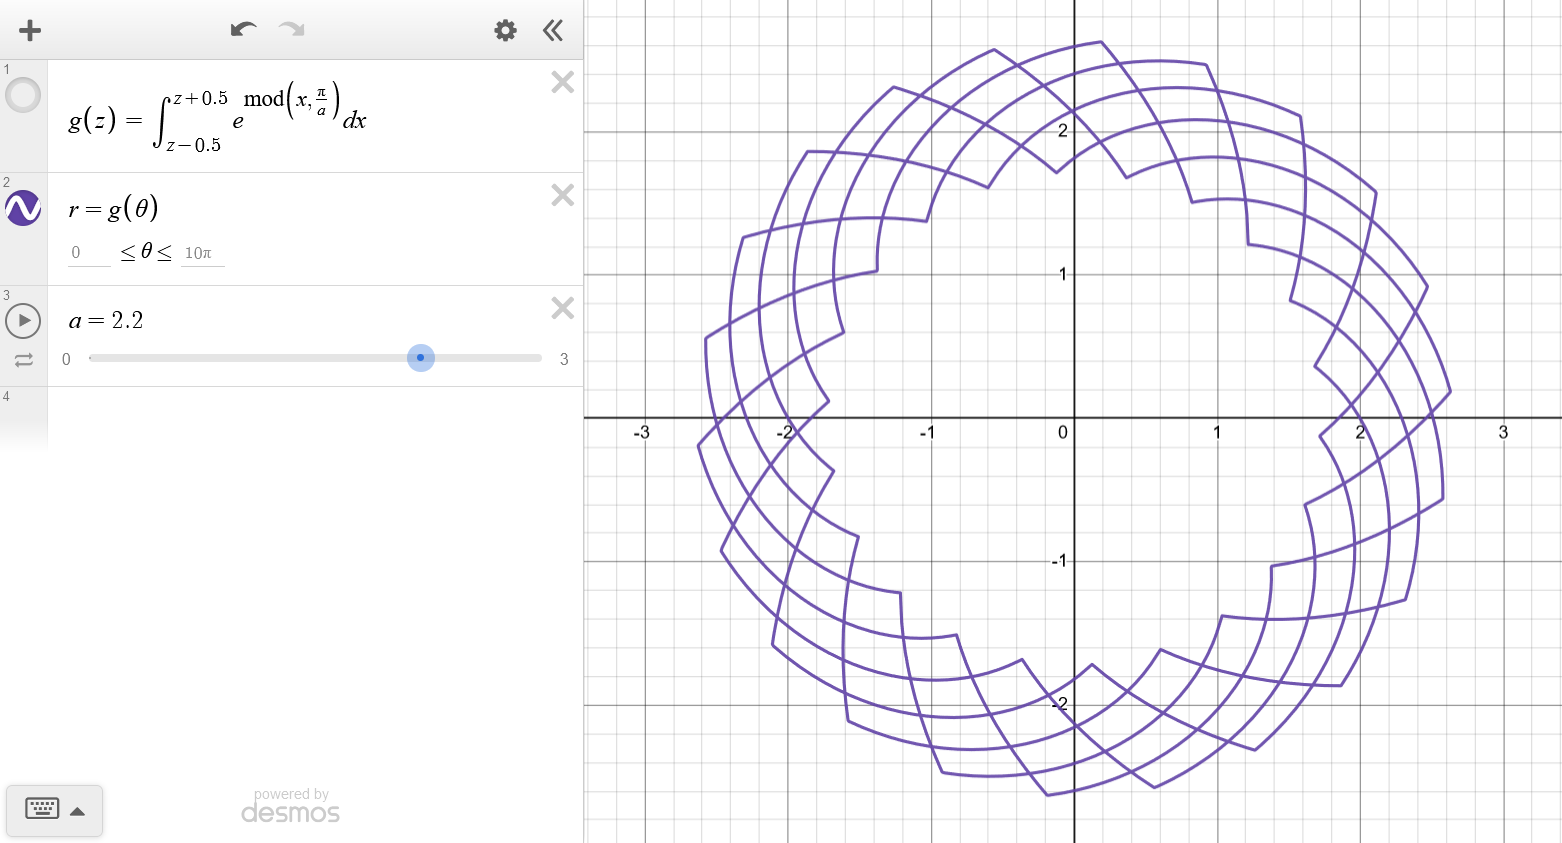
\includegraphics[width=0.45\textwidth]{desmos_advertisement_lol}
		
		\footnotesize \raggedright Desmos, a powerful graphing calculator that allows you to plot various kinds of functions.
	\end{wrapfigure}
	We are familiar with graphs/plots, an ingenious technique that allows us to visualize how a function $f(x)$ varies as $x$ changes. As you can see above, most graphs that we have dealt with until now have been 2-dimensional (i.e there are two axes). Typically, the horizontal $x$-axis is the range of inputs (called domain), and the vertical $y$-axis represents the range of outputs(called range) of some function for all values of x. We signify this by stating $y = f(x)$, where $f$ is some arbitrary function.\\[1em]
	But starting from now, a function may have more than one input. So higher dimensional graphs are necessary. Here is a picture of a 3D graph representing a real valued function of two variables. 
	\begin{center}
		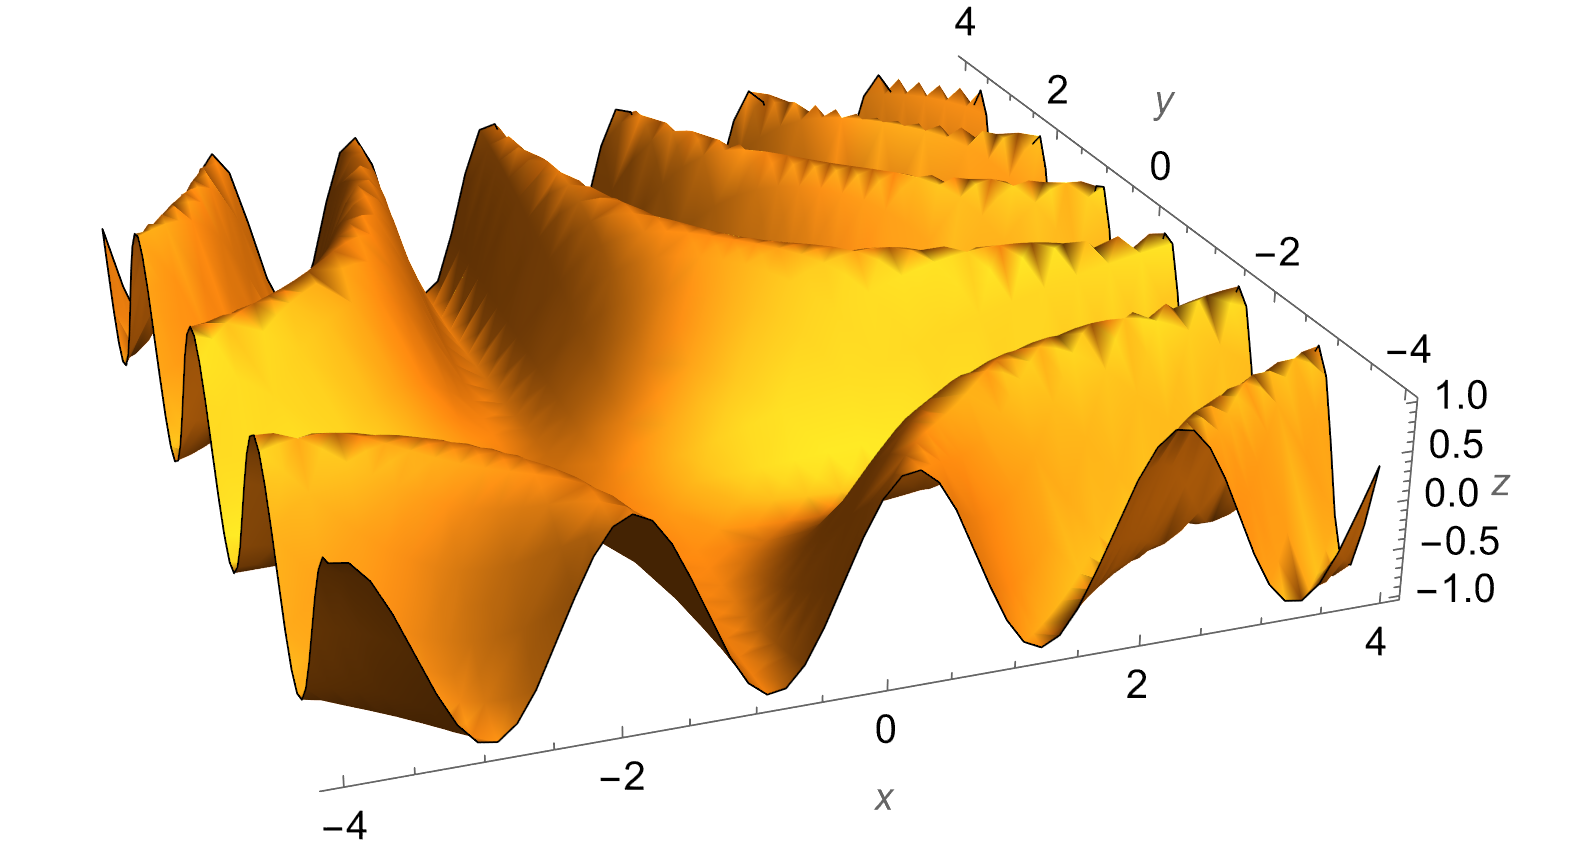
\includegraphics[width=15cm]{3d-graph_1}
		
		\footnotesize The plot of $z = \sin(xy + x + y)$
	\end{center}
	The bottom two axes $x$ and $y$ represent the input \textit{plane} representing the entire area over which the function $f(x, y)$ may vary. The output is cast onto the z-axis(a vertical \textit{line}) and the colored \textit{surface} you can see represents the set of all 3-tuples $(x,y,z)$ such that $z = f(x, y)$. The entire graph is a 3-dimensional \textit{space}. It is important to get a feel for these terminologies and be able to discuss them in order to communicate effectively. 
	
	But now we face a problem. A function with 3 inputs $f(x, y, z)$ will require 3+1=4 dimensions to be graphed properly. The more inputs a real-valued function has, the more complex the graph will become. Hence, we are basically unable to graphically visualize and imagine functions of arbitrary dimensions. Abstract thinking and strong imagination are of paramount importance if one wishes to interpret/visualize these higher dimensional functions in any meaningful way. 
	
	\subsubsection{Level sets}
	The world we live in is 3 dimensional {\footnotesize(well, spatially...)}. Therefore, it is not surprising that most of the problems that we need to solve and hence much of multivariate calculus, focuses heavily on 3 and 4-dimensional real-valued functions {\footnotesize (you'll see this in Vector Calculus, wait...)} as we try to model real-world scenarios for mathematical analysis. 
	
	We already saw in the previous section that functions with 3 inputs $w = f(x, y, z)$ are impossible to visualize properly because they require 4 dimensions. And it's not exactly an easy feat to generate 3D plots of functions either. Computationally expensive, hard to move around and view properly, and hardware limitations mean that these 3D graphs should serve as a means of gaining intuition but not some rigorous and analytical tool that we can use to make judgements regarding these functions.
	
	Fortunately, we can use a technique that reduces the number of dimensions as long as we care only about a specific value of the function's output. Let's have a look at level curves and surfaces.
	
	\paragraph{Level curve} The level curve of $f(x, y)$ at $c$ is the set of all $(x, y)$ such that $f(x, y) = c$.
	\begin{equation*}
		\left\{ (x, y) \mid f(x, y) = c \right\} 
	\end{equation*}
	This turns a multivariate function of 3 dimensions into an implicit function of 2 dimensions. 
	
	Let us try to understand what this means geometrically. Suppose $z=f(x, y)$, and let's take a simple function $f(x, y) = x^2 + y^2$. 
	
	\begin{center}
		\begin{tabular}{l l}
			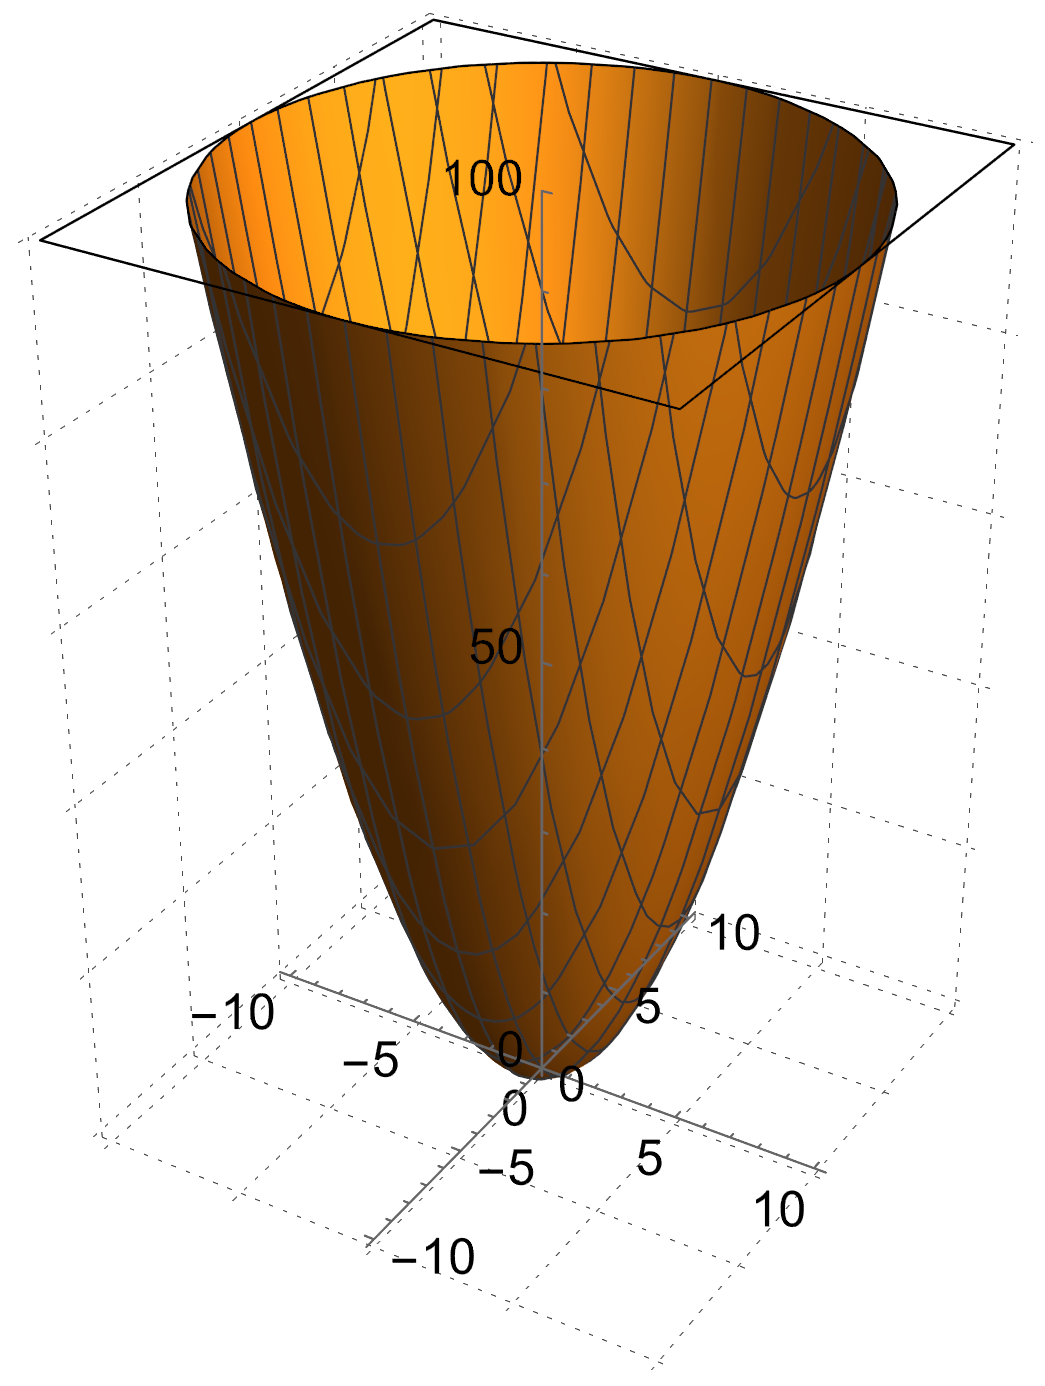
\includegraphics[width=0.5\textwidth]{3d-graph_2} & 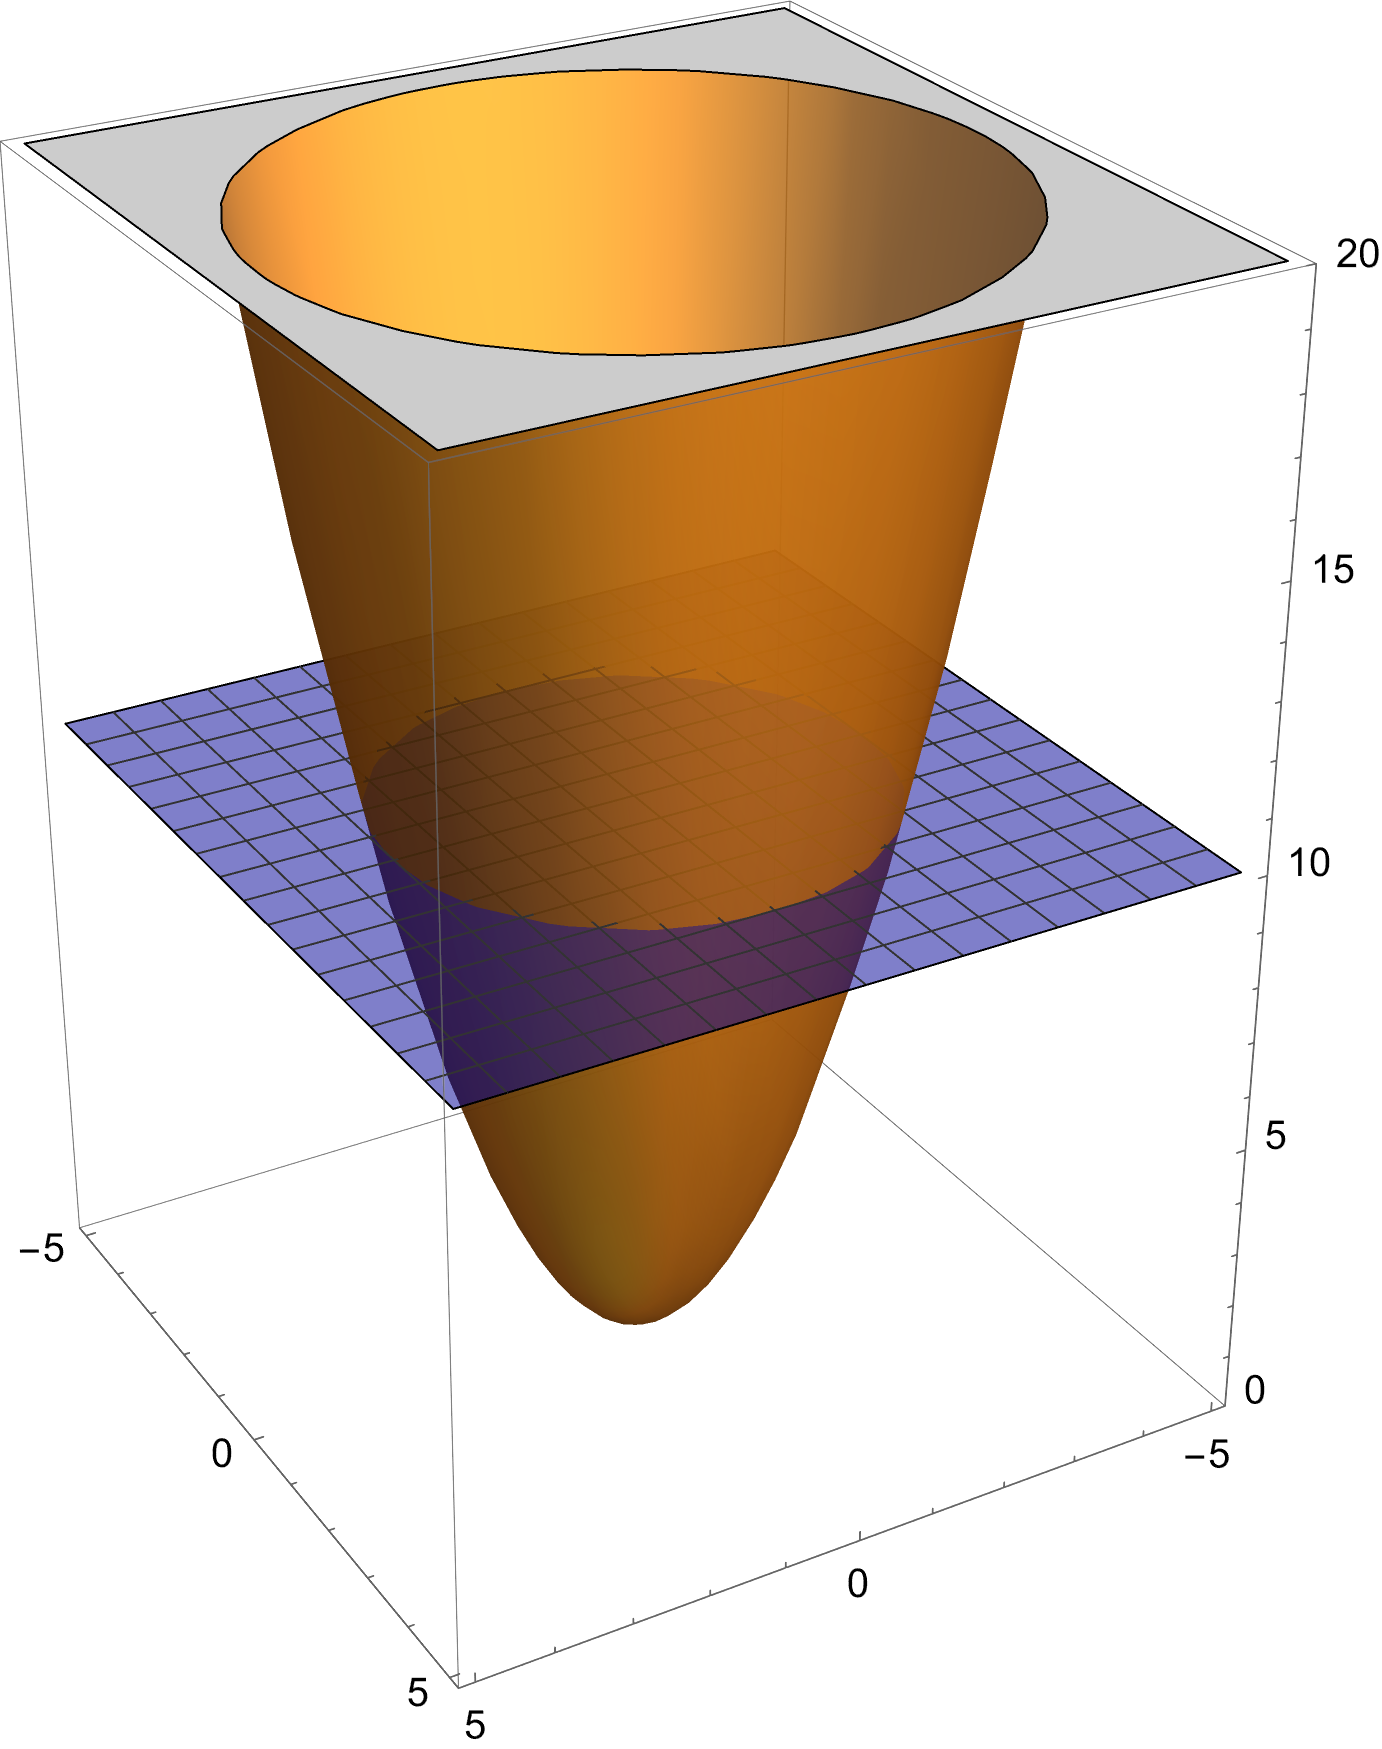
\includegraphics[width=0.5\textwidth]{3d-graph_3}\\
			$\bullet$ \footnotesize The 3D plot of $z = x^2 + y^2$ from $x: [-10, 10]$, $y: [-10, 10]$ & $\bullet$ \footnotesize The plane $z = 10$ (blue) and the surface $z = x^2 + y^2$ (orange). The points where the two surfaces intersect can be thought of as the level curve of $f(x, y) = x^2 + y^2$ at $10$.
		\end{tabular}
	\end{center}
	You can see that $f(x, y) = c$, i.e the level curve, can be thought of as the intersection between the plane $z = c$ and the surface $z = f(x, y)$. The plane $z=c$ is parallel to the $xy$-plane. Any point on the plane has coordinates $(x, y, c)$ where $x$ and $y$ are free variables. For the above image, the intersection between these two surfaces, $z = 10$ and $z = x^2 + y^2$, can be described as 
	\begin{equation*}
		\left\{ (x, y) \mid x^2 + y^2 = 10 \right\} 
	\end{equation*}
	Which describes a circle on the $xy$-plane of radius $\sqrt{10}$ centered at the origin.
	 
	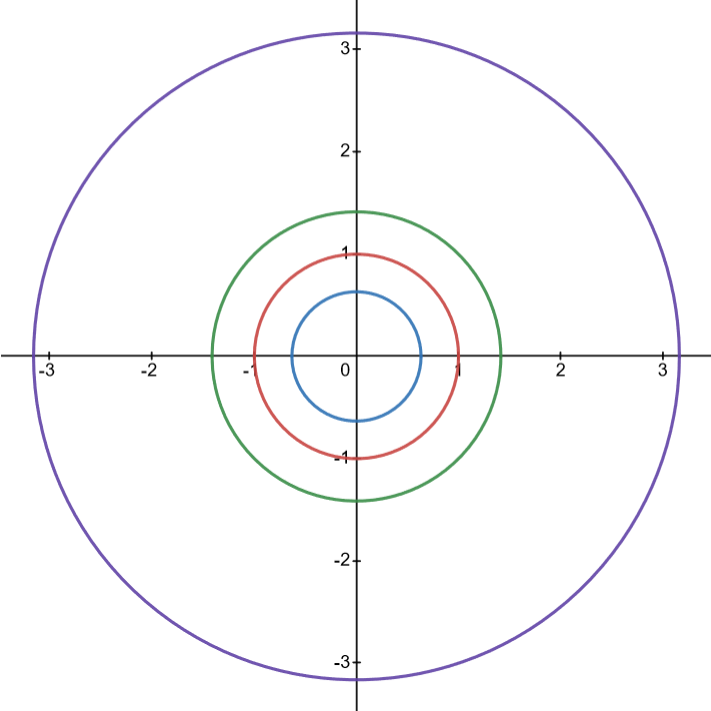
\includegraphics[width=10cm]{level_curve1}
	\begin{textblock*}{7cm}(11.5cm, -5.8cm)
		\small \noindent Some level curves of $z=x^2 + y^2$ at,\\[-2em]
		
		\begin{tasks}(1)
			\task $c = 0.4$ (blue)
			\task $c = 1$ (red)
			\task $c = 2$ (green)
			\task $c = 10$ (purple)
		\end{tasks}
	\end{textblock*}

	\paragraph{Level surfaces} The level surface of $f(x, y, z)$ at $c$ is the set of all $(x, y, z)$ such that $f(x, y, z) = c$.
	\begin{equation*}
		\left\{ (x, y, z) \mid f(x, y, z) = c \right\} 
	\end{equation*}
	This turns a multivariate function of 4 dimensions into an implicit function of 3 dimensions. We can now generalize and say that for higher dimensions, ...
	
	\paragraph{Level set} The level set of $f(\mathbf{v})$ at $c$ is the set of all $n$-tuples such that $f(\mathbf{v}) = c$.
	\begin{equation*}
		\left\{ \mathbf{v} \in \mathbb{R}^n \mid f(\mathbf{v}) = c \right\} 
	\end{equation*}
	This turns a multivariate function $f: \mathbb{R}^n \rightarrow \mathbb{R}$ of $n$ dimensions into an implicit function of $n-1$ dimensions. The number of dimensions has been reduced by $1$ because there are only $n-1$ free variables. 
	
	In the future we will sometimes be making references to level sets to describe ...
	
	\pagebreak
	\section{Differentiation in Multivariate Calculus}
	
	
	\section{Integration in Multivariate Calculus}
	We should already be familiar with single-variable integration. Indeed, the area under a curve $y=f(x)$ from $x = a$ to $x=b$ is given by,
	
	\begin{center}
		\begin{tabular}{c c}
			\begin{minipage}[c][5cm][c]{6cm}
				\begin{equation*}
					A = \int_a^b f(x) \odif{x}
				\end{equation*} 
			\end{minipage}
			&
			\begin{minipage}[c][6cm][c]{6cm}
				\begin{tikzpicture}[baseline]
					\fill [gray!30, domain=0.5:2.7, variable=\x]
					(0.5, 0)
					-- plot ({\x}, {0.8*\x*\x*\x - 3.5*\x*\x + 4.6*\x + 0.9})
					-- (2.7, 0)
					-- cycle;
					
					\draw [thick] [->] (0,0)--(5,0) node[right, below] {$x$};
					%\foreach \x in {0,...,4}
					%\draw[xshift=\x cm, thick] (0pt,-1pt)--(0pt,1pt) node[below] {$\x$};
					
					\draw [thick] [->] (0,0)--(0,5) node[above, left] {$y$};
					%\foreach \y in {0,...,3}  % loop that draws numbers on the axes
					%\draw[yshift=\y cm, thick] (-1pt,0pt)--(1pt,0pt) node[left] {$\y$};
					
					\draw[xshift=0.5 cm, thick] (0pt,-1pt)--(0pt,1pt) node[below] {\vphantom{b}$a$};
					\draw[xshift=2.7 cm, thick] (0pt,-1pt)--(0pt,1pt) node[below] {\vphantom{b}$b$};
					
					\draw [domain=0:3, variable=\x]
					plot ({\x}, {0.8*\x*\x*\x - 3.5*\x*\x + 4.6*\x + 0.9}) node[right] at (1.2,1.5) {\Large $A$};
				\end{tikzpicture}
			\end{minipage}
		\end{tabular}
	\end{center}
	
	We now extend this idea to multivariate functions. If $z = f(x, y)$, then the inputs of this function could be imagined as a plane $(x,y)$. Letting the output $z$ be represented on a separate axis, we then see that a \textit{volume} is covered by the surface $z= f(x, y)$ and the plane formed by the $x$ and $y$ axes. 
	\begin{center}
		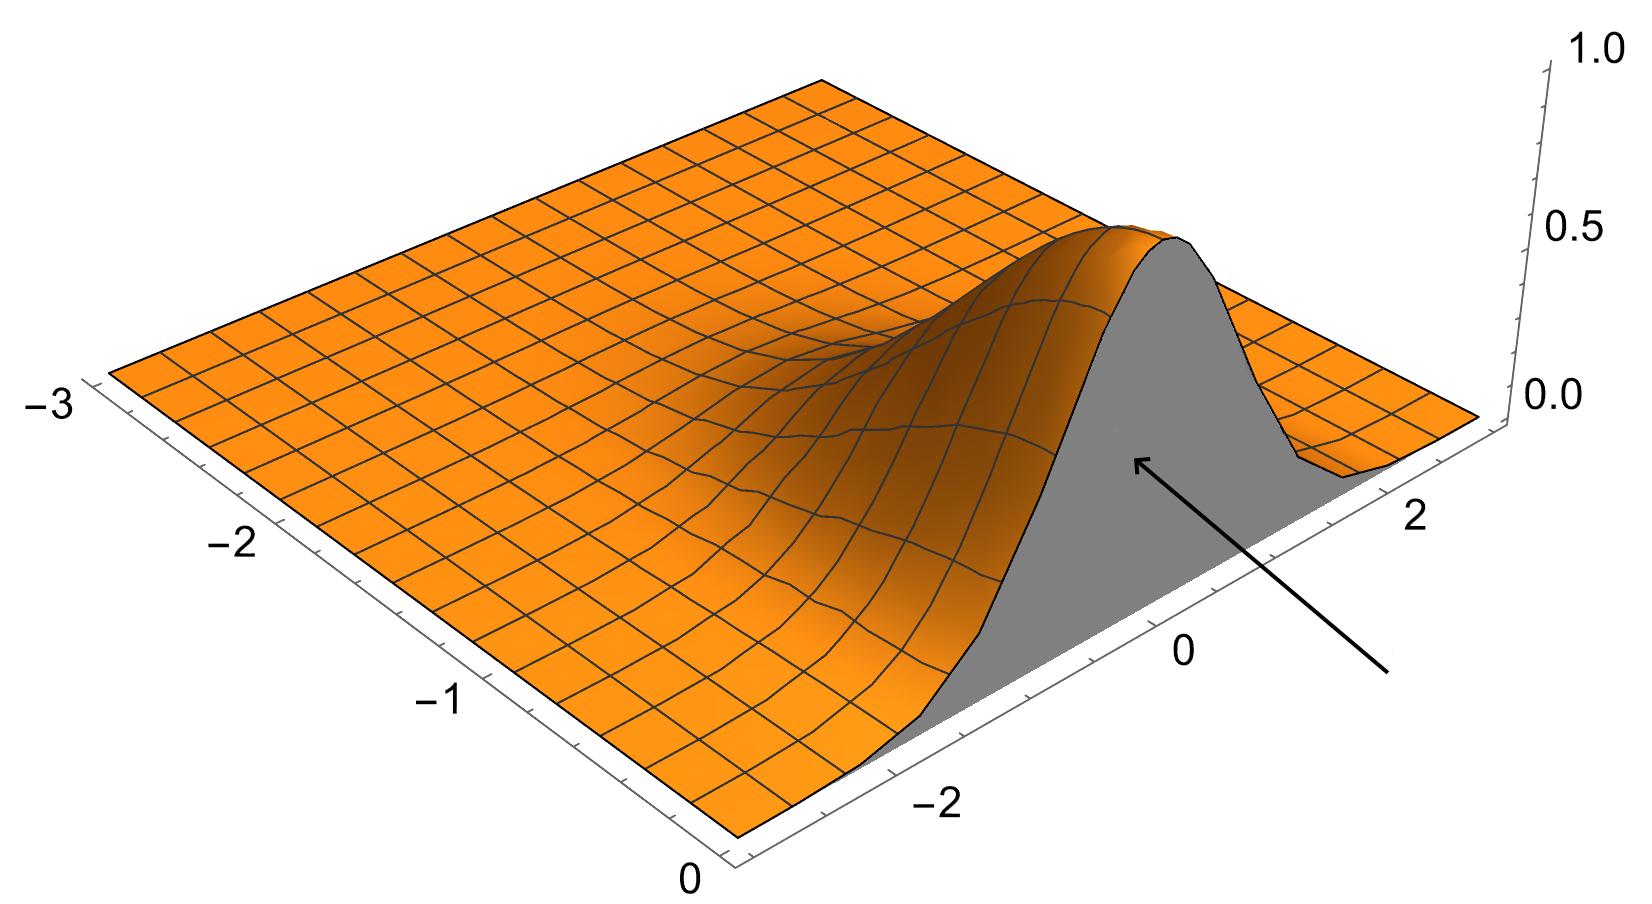
\includegraphics[width=12cm]{3d_plot_volume_under_blue}
		\begin{textblock*}{2cm}(13.8cm, -1.8cm)
			Volume!
		\end{textblock*}
	\end{center}
	$\Delta x$ and $\Delta y$ are small infinitesimal changes to the inputs $x$ and $y$ respectively. Then, considering some point $P(x_0, y_0)$, if we move in any direction, the corresponding change may be in both $\Delta x$ and $\Delta y$. 
	
	
	\section{Vector Calculus}
	\subsubsection{Parametrization} An arbitrary path in $\mathbb{R}^n$ can be traced out from a beginning to an end using parameters, so
	\begin{equation*}
		r: \mathbb{R} \rightarrow \mathbb{R}^n \qquad\qquad \vec{r}(t) = g(t) \hat{i} + h(t) \hat{j}
	\end{equation*}
	
	\section{Stuff I felt like doing before others}
	DRAFT -- delet dis later obvs xd pls i cri pls delet :(((
	
	\begin{example}{Prove that the volume of a sphere is $\frac{4}{3}\pi r^3$}{}
		A very interesting question: surely this is a formula that everyone is familiar with from school. Back then you had to memorize this expression, but haven't you ever wondered where this formula came from or why this is true? 
		
		Now that we know we can evaluate the volume of any arbitrary shape by describing the region it occupies in space and evaluating the triple integral w.r.t. the coordinate axes. Look at the image to see the region we will be integrating over.
		\begin{equation*}
			V = \iiint_{\text{\tiny Sphere}} 1 \odif{x, y, z}
		\end{equation*}
		\begin{equation*}
			\begin{split}
				V & = \iiint_{\text{\tiny Sphere}} r^2 \sin{\phi} \odif{r, \phi, \theta} \\
				& \implies \int_{\scriptscriptstyle \theta=0}^{\scriptscriptstyle \theta=2\pi} \int_{\scriptscriptstyle\phi=0}^{\scriptscriptstyle\phi=\pi} \int_{\scriptscriptstyle r=0}^{\scriptscriptstyle r=R} r^2 \sin{\phi} \odif{r, \phi, \theta} \\
				& \implies \int_{\scriptscriptstyle\theta=0}^{\scriptscriptstyle\theta=2\pi} \int_{\scriptscriptstyle\phi=0}^{\scriptscriptstyle\phi=\pi} \sin{\phi} \left[\frac{r^3}{3}\right]_0^R \odif{\phi, \theta} \\
				& \implies \frac{R^3}{3} \int_{\scriptscriptstyle\theta=0}^{\scriptscriptstyle\theta=2\pi} \left[-\cos{\phi}\right]_0^\pi \odif{\theta} \\
				& \implies \frac{2}{3} R^3 \int_{\scriptscriptstyle\theta=0}^{\scriptscriptstyle\theta=2\pi} \odif{\theta} \\
				& \implies \frac{2}{3} R^3 \left[\theta\right]_0^{2\pi} \\
				& \implies \frac{4}{3} \pi R^3
			\end{split}
		\end{equation*}
		
	\end{example}
\end{document}
